\documentclass[11pt]{article}

% --- Packages ---
\usepackage[utf8]{inputenc}
\usepackage[T1]{fontenc}
\usepackage{lmodern}
\usepackage[margin=1in]{geometry}
\usepackage{graphicx}
\usepackage{booktabs}
\usepackage{amsmath}
\usepackage{siunitx}
\usepackage{authblk}
\usepackage[hidelinks]{hyperref}
\usepackage[numbers,sort&compress]{natbib}
\usepackage{caption}
\captionsetup{labelfont=bf,font=small}
\graphicspath{{figures/}}

% Structure follows Scientific Reports: Introduction, Results, Discussion, Methods.

\title{\textbf{Does clinical context help a chest-radiograph pneumonia model?\\
A time-safe multimodal study with multi-seed reproducibility\\ and missing-data cautions}}

\author[1]{Yazan Al-Dabain}
\affil[1]{Department of Data Science and Engineering, Faculty of Informatics,
E\"otv\"os Lor\'and University, Budapest, Hungary}
\date{}

\begin{document}
\maketitle

\begin{abstract}
\noindent
Emergency-department (ED) triage produces structured clinical data before chest
imaging, raising the question of whether fusing that context with the chest
radiograph (CXR) improves automated pneumonia detection. We build a temporally
safe multimodal cohort from MIMIC-CXR-JPG, MIMIC-IV and MIMIC-IV-ED, anchoring
every feature at the CXR acquisition time $t_0$ and admitting only measurements
resulted at or before $t_0$. On a patient-level temporal split (test $n=1{,}075$,
prevalence 45.3\%), a fine-tuned DenseNet-121 reaches AUROC $0.737\pm0.003$ across
five training seeds, far above triage-only baselines (logistic regression 0.606,
XGBoost 0.611). Adding triage vitals leaves discrimination unchanged
($\Delta$AUROC $+0.004\pm0.009$, within a pre-specified $\pm0.05$ non-inferiority
margin). Two reproducibility findings dominate. First, a calibration advantage
reported from a single checkpoint (expected calibration error, ECE, 0.040 vs
0.067) shrinks to $\Delta$ECE $-0.013\pm0.016$ across seeds---single-seed
evaluation overstated the effect roughly twofold. Second, adding a broad early-lab
panel produces a small, seed-consistent AUROC gain ($+0.009\pm0.005$, 5/5 seeds),
but an ablation shows this gain is reproduced exactly by the lab \emph{missingness
indicators alone}, with no contribution from the lab values---the apparent benefit
is missing-data structure, not chemistry, and is not attributable to leakage
(temporal, split and preprocessing audits all clean). On external validation
against 112{,}120 NIH ChestX-ray14 radiographs, discrimination transfers with
minimal loss (AUROC $0.722\pm0.005$, $-0.016$ vs internal). We further report
subgroup performance gaps not closed by fusion, that a modern CXR foundation
backbone does not outperform the task-tuned model, and that CRP and procalcitonin
are available before imaging in under 1\% of studies. The chest radiograph carries
the discriminative signal for radiographic pneumonia; immediately available
clinical context does not reliably add discrimination, and naive multimodal fusion
can appear beneficial for reasons that will not generalise.
\end{abstract}

\section*{Introduction}
Pneumonia is a leading cause of ED presentation and admission, and the chest
radiograph remains central to its diagnosis~\citep{metlay2019idsa}. Deep-learning
CXR classifiers approach radiologist-level performance on several findings, and a
substantial literature proposes fusing imaging with structured clinical
data~\citep{acosta2022multimodal,hayat2022medfuse,soenksen2022multimodal}. Three
methodological issues recur in that literature and motivate this study.
First, \textbf{temporal safety}: clinical variables are frequently included without
verifying they were available at prediction time, risking optimistic leakage.
Second, \textbf{single-seed reporting}: calibration and small discrimination effects
are often reported from one training run, although both are sensitive to training
stochasticity~\citep{guo2017calibration,nixon2019measuring}. Third,
\textbf{missing data}: clinical inputs in the ED are heavily and non-randomly
missing, so a model can exploit \emph{whether} a measurement exists rather than its
value. We address a deliberately conditional question---\emph{when, if ever, does
immediately available clinical context help a CXR pneumonia model?}---under strict
time-safety, with multi-seed replication and explicit missing-data and leakage
audits. Our contribution is not a new architecture but a rigorous, reproducible
evaluation and two transferable cautions for clinical multimodal fusion, reported
in line with prediction-model and medical-imaging guidance~\citep{collins2024tripodai,tejani2024claim}.

\section*{Results}

\subsection*{The image dominates; fusion is discrimination-neutral}
Across five seeds (test $n=1{,}075$; Table~\ref{tab:main}, Fig.~\ref{fig:multiseed}),
both CXR models beat triage-only baselines by more than 12 AUROC points. Adding
triage vitals does not change discrimination (concat $-$ image $\Delta$AUROC
$+0.004\pm0.009$; lower bound of the effect well inside the $-0.05$ non-inferiority
margin~\citep{piaggio2012noninferiority}). Attention fusion matches image AUROC but
is severely and variably miscalibrated (ECE $0.076\pm0.042$).

\begin{table}[htbp]
\centering
\caption{Multi-seed test-set performance (mean $\pm$ SD over 5 seeds; $n=1{,}075$;
prevalence 45.3\%). Clinical baselines are single-fit.}
\label{tab:main}
\small
\begin{tabular}{@{}lcccc@{}}
\toprule
Model & AUROC & AUPRC & ECE & Brier \\
\midrule
Image-only DenseNet-121            & $0.737\pm0.003$ & $0.719\pm0.004$ & $0.053\pm0.008$ & $0.207\pm0.001$ \\
Multimodal --- concat (triage)     & $0.741\pm0.006$ & $0.715\pm0.005$ & $0.040\pm0.014$ & $0.205\pm0.002$ \\
Multimodal --- attention (triage)  & $0.738\pm0.006$ & $0.713\pm0.012$ & $0.076\pm0.042$ & $0.212\pm0.010$ \\
Multimodal --- concat (+labs)      & $0.747\pm0.004$ & $0.724\pm0.004$ & $0.043\pm0.011$ & $0.203\pm0.002$ \\
Logistic regression (triage)       & 0.606 & 0.548 & 0.037 & 0.242 \\
XGBoost (triage)                   & 0.611 & 0.567 & 0.046 & 0.241 \\
\bottomrule
\end{tabular}
\end{table}

\begin{figure}[htbp]
\centering
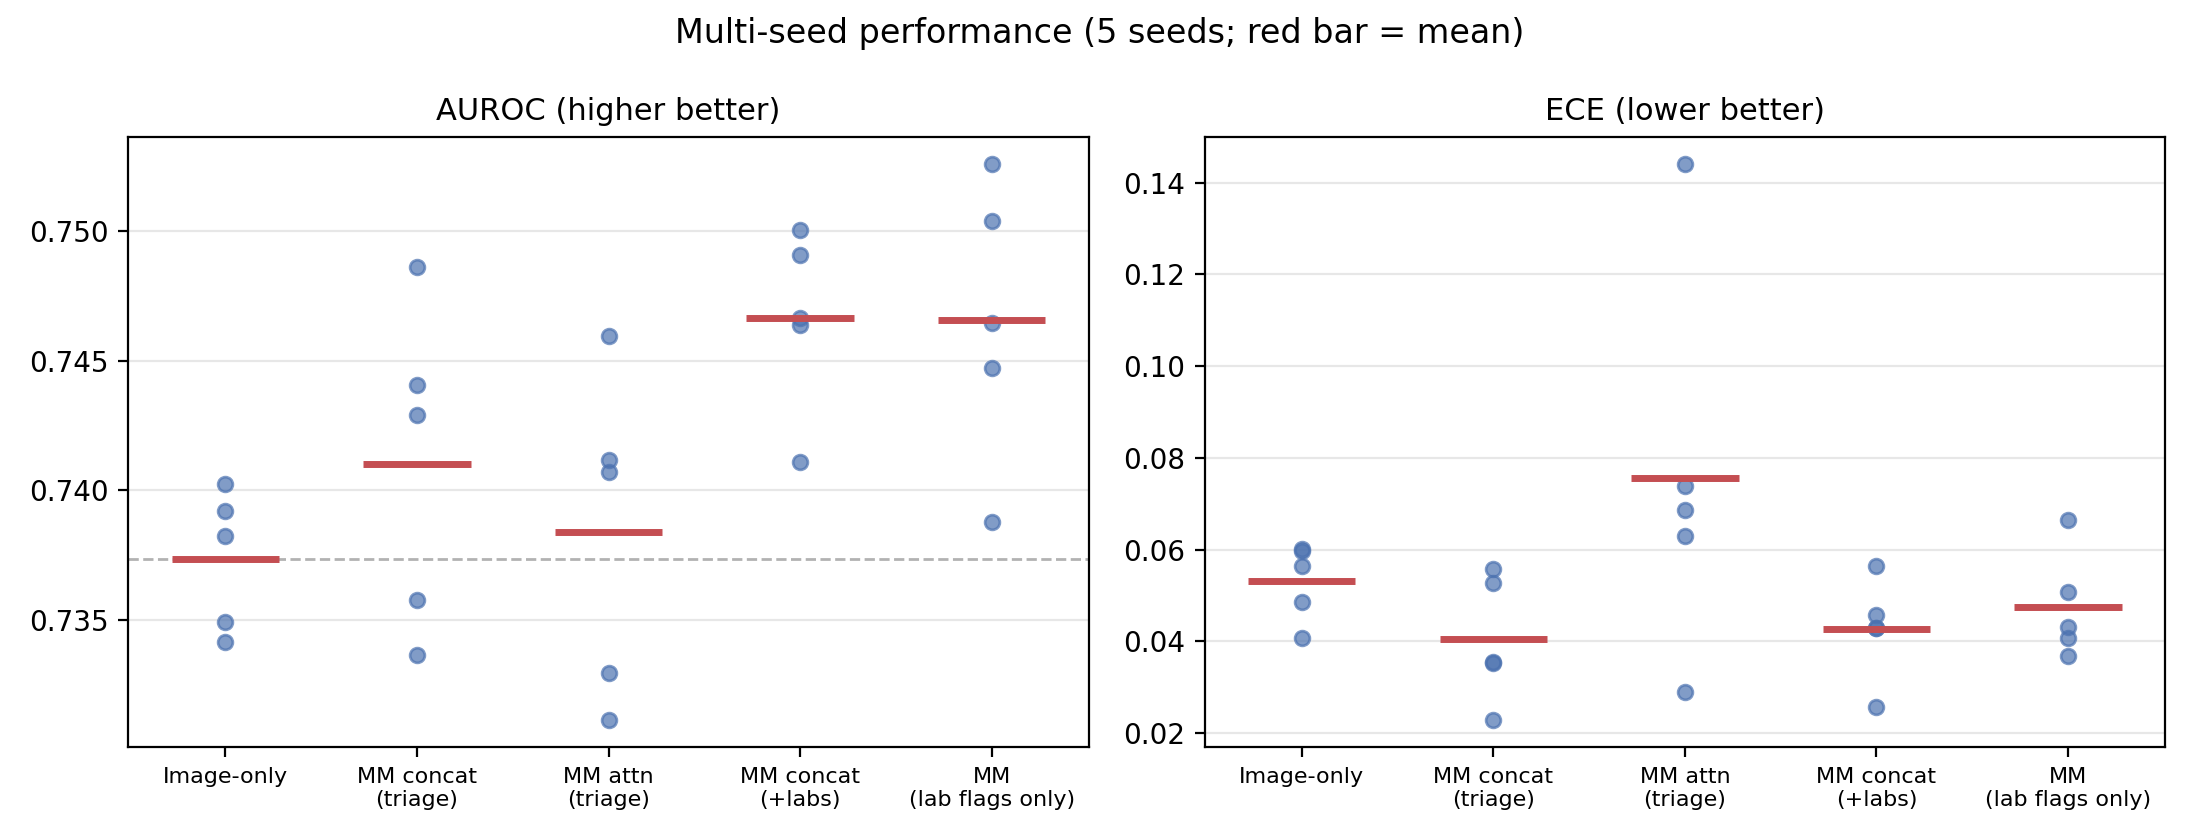
\includegraphics[width=0.95\textwidth]{fig1_multiseed_metrics.png}
\caption{Per-model AUROC and ECE across five seeds (points, seeds; red bar, mean).
Discrimination is stable; the image-only ECE alone varies substantially by seed.}
\label{fig:multiseed}
\end{figure}

\begin{figure}[htbp]
\centering
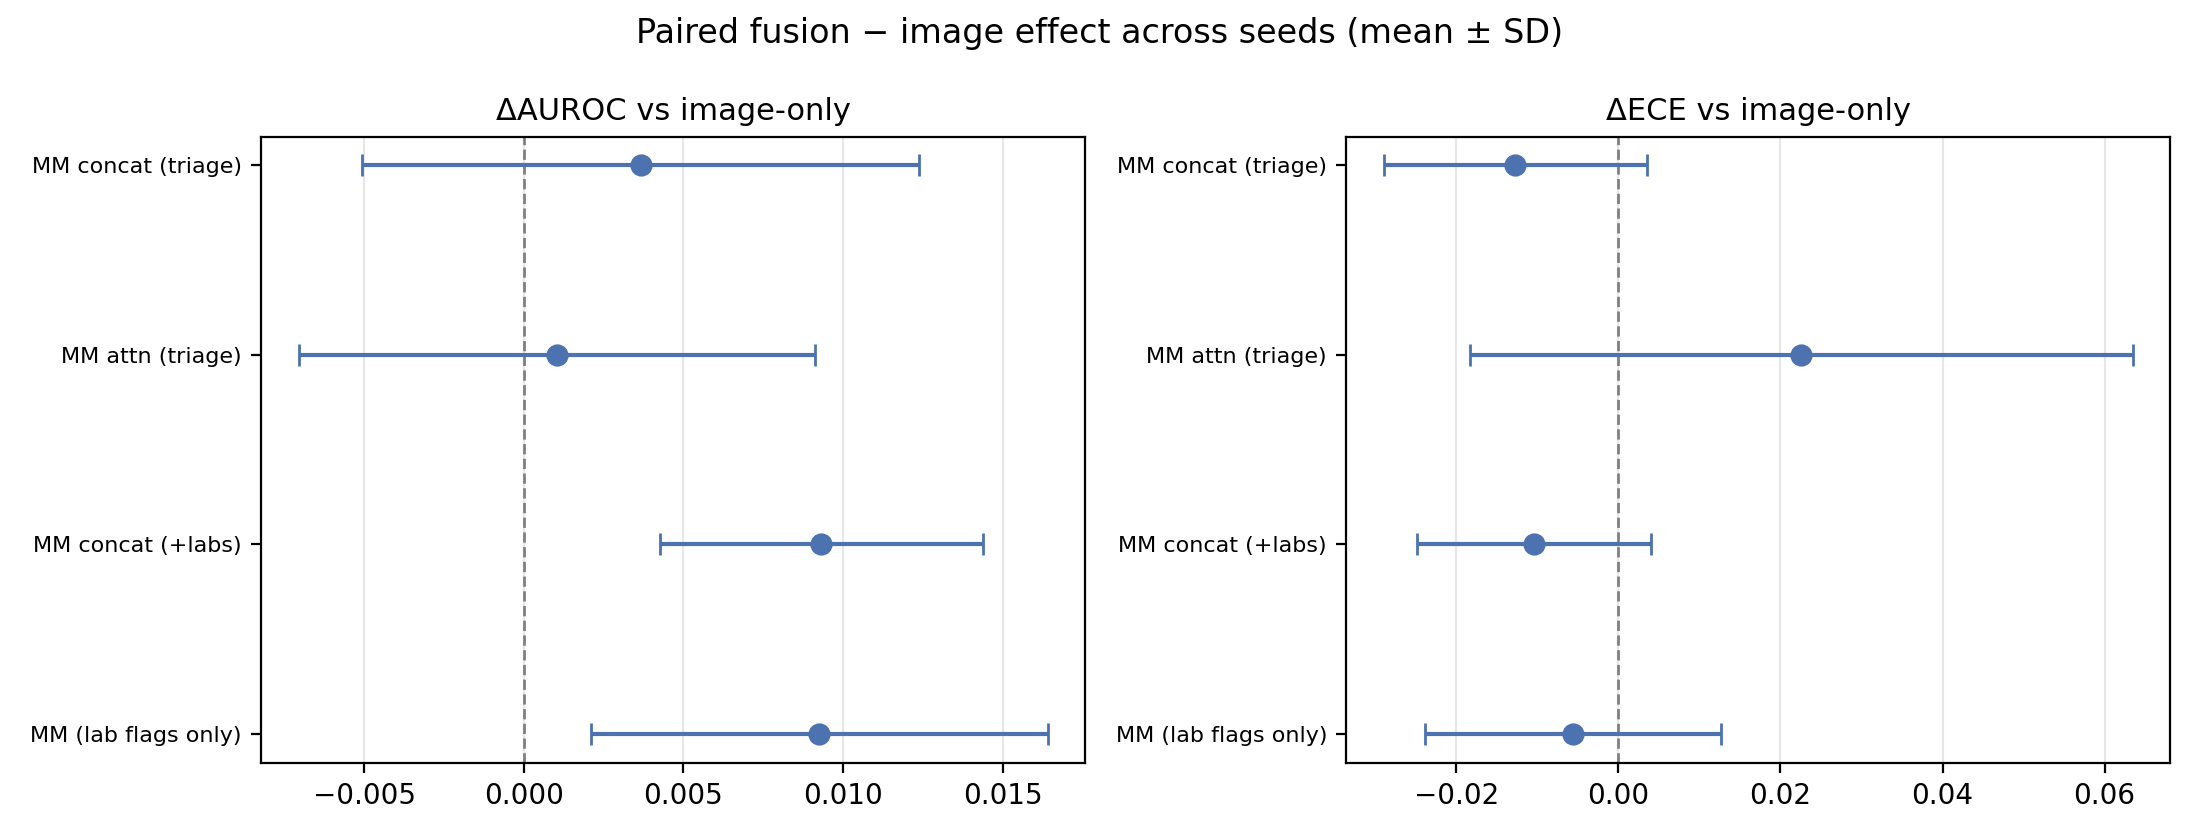
\includegraphics[width=0.95\textwidth]{fig2_paired_deltas.png}
\caption{Paired fusion $-$ image effects across seeds (mean $\pm$ SD). Every effect
straddles zero; the labs and lab-flags-only deltas are identical, indicating the
labs effect is driven by missingness rather than lab values.}
\label{fig:deltas}
\end{figure}

\subsection*{Reproducibility caution 1: single-seed evaluation inflates the calibration effect}
A single checkpoint suggested the concat model was markedly better calibrated (ECE
0.040 vs 0.067, a 40\% reduction). Across seeds the image-only ECE alone ranges
0.041--0.060, and the paired advantage shrinks to $\Delta$ECE $-0.013\pm0.016$ (4/5
seeds favour concat; range crosses zero). The single-seed estimate overstated the
benefit roughly twofold. The effect is also binning-dependent (Fig.~\ref{fig:ece};
$\Delta$ECE $-0.005$ at 5 bins to $-0.013$ at 10 bins~\citep{nixon2019measuring}).
Brier scores are essentially unchanged, so any effect is distributional alignment,
not refinement.

\subsection*{Reproducibility caution 2: the labs ``benefit'' is missing-data structure}
Appending early labs gives the only seed-consistent AUROC gain (labs $-$ image
$+0.009\pm0.005$, 5/5 seeds, range excludes zero). Three analyses show this is not
a genuine chemistry signal and not leakage. \emph{Ablation:} a model using lab
\emph{missingness flags only} (no values) reproduces the gain exactly (flags $-$
image $+0.009$; Fig.~\ref{fig:deltas}); the lab values add nothing further to
discrimination. \emph{Subcohort:} on the 269 test studies that actually have labs,
discrimination is tied (labs 0.778 vs image 0.776). \emph{Leakage audit:} 0 of
314{,}145 lab measurements post-$t_0$; 0 cross-split subjects; preprocessing fit on
train only; the ``any lab drawn'' indicator has near-null univariate AUROC (0.464).
The gain therefore reflects the weak complementary signal of \emph{whether}
bloodwork was ordered, is small, and lies within the patient-level bootstrap CI---a
concrete caution that multimodal fusion with heavily missing inputs can appear
beneficial for reasons that will not transfer.

\subsection*{Clinical availability of labs}
Under time-safe matching, only 25.4\% of ED-anchored CXR studies (272/1{,}075 test)
have any resolved lab at or before imaging; CBC and metabolic panels reach $\sim$25\%,
but CRP and procalcitonin---the most pneumonia-specific markers---are present in
0.5\% and 0.6\% (Fig.~\ref{fig:labcov}). At the moment of imaging, the informative
labs are essentially unavailable.

\subsection*{Operating points, subgroups, and modern backbone}
At a fixed sensitivity of 0.90, specificity is 0.31 (image) vs 0.32 (concat); at
0.95, 0.17 vs 0.18---clinically equivalent. Subgroup AUROC reveals disparities not
closed by fusion (Fig.~\ref{fig:subgroup}): male 0.77 vs female 0.71; White 0.75,
Black 0.71, Hispanic 0.64 (small strata, wide CIs); PA view 0.75 vs AP
0.72~\citep{seyyedkalantari2021underdiagnosis,larrazabal2020gender}. A
CheXpert-trained DenseNet-121~\citep{cohen2022torchxrayvision}, used zero-shot
(AUROC 0.667) or as a frozen-feature linear probe (0.687), does not outperform our
task-tuned model (0.737).

\subsection*{External validation}
We evaluated the image models on all 112{,}120 radiographs of NIH
ChestX-ray14~\citep{wang2017chestxray} (a different institution, scanner population
and label pipeline; 1{,}431 pneumonia-positive, prevalence 1.28\%). Discrimination
transfers with minimal loss: AUROC $0.722\pm0.005$ across five seeds (ensemble
0.726), only 0.016 below the internal 0.737 (Fig.~\ref{fig:external}). As expected
under the large prevalence shift ($45\%\to1.3\%$), prevalence-dependent metrics
degrade (AUPRC 0.030, ECE 0.44) because probabilities are calibrated to the internal
base rate; AUROC is the appropriate prevalence-independent cross-dataset metric, and
it holds despite domain shift and NLP-derived external labels.

\begin{figure}[htbp]
\centering
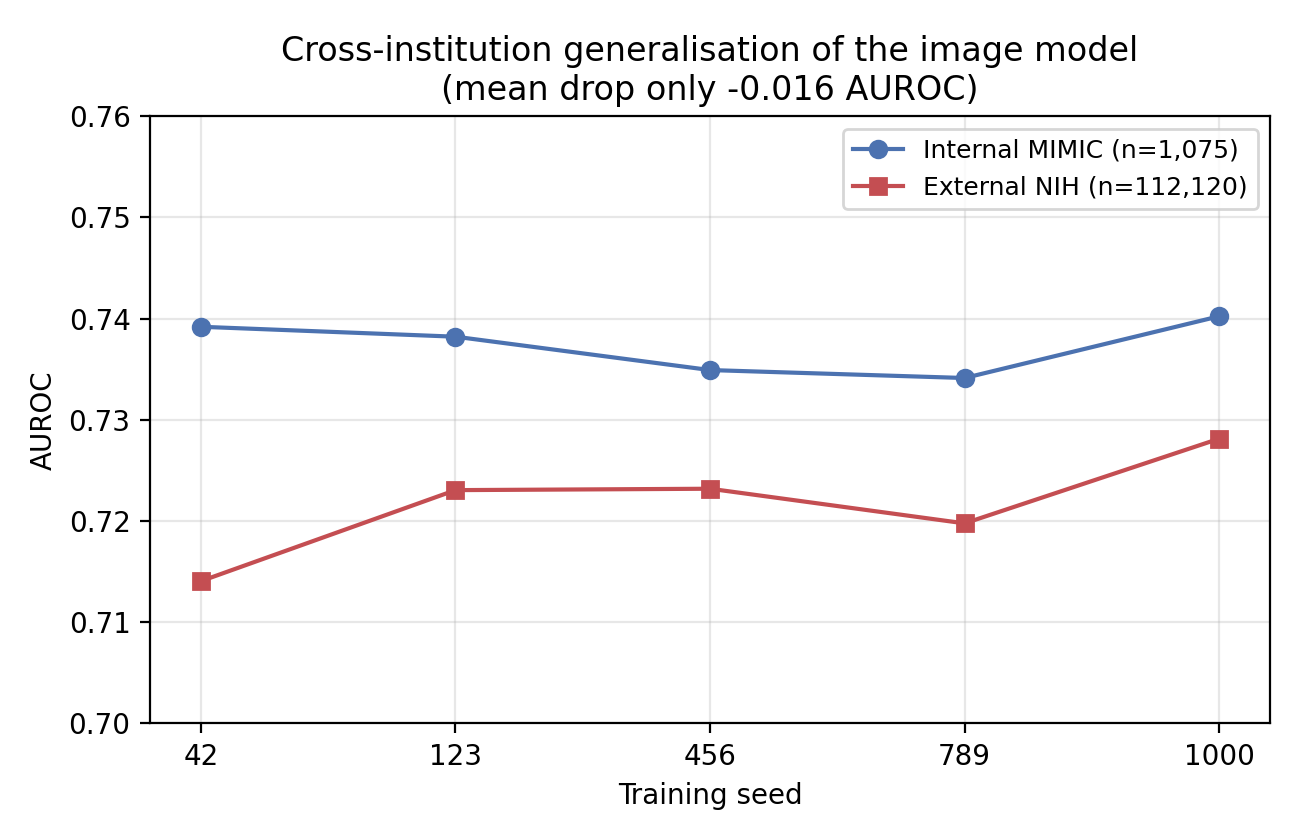
\includegraphics[width=0.6\textwidth]{fig6_external_nih.png}
\caption{Cross-institution generalisation: per-seed AUROC on internal MIMIC
($n=1{,}075$) vs external NIH ChestX-ray14 ($n=112{,}120$); mean drop $-0.016$.}
\label{fig:external}
\end{figure}

\section*{Discussion}
The chest radiograph carries the discriminative signal for radiographic pneumonia in
this ED cohort; immediately available structured clinical context---triage vitals,
and even a broad early-lab panel---does not add reliable discrimination, and the image
model generalises externally with minimal loss. This is a well-powered negative answer
to a specific, clinically motivated question, accompanied by two transferable
methodological cautions. Reporting calibration or small discrimination effects from a
single training run can overstate them (here $\sim2\times$); multi-seed replication
should be standard. And where clinical inputs are heavily and non-randomly missing, a
multimodal model can exploit missingness structure and present a spurious benefit that
neither reflects the measured values nor generalises---a failure mode distinct from
data leakage, which our audits explicitly excluded.

\paragraph{Limitations.} Training and multimodal evaluation are single-institution
(MIMIC) and retrospective; external validation confirms the image branch generalises to
NIH but is necessarily limited to imaging, as no external dataset links ED triage to the
CXR, and probabilities require recalibration to the target base rate before deployment
(the \texttt{u\_ignore} policy also raises internal evaluation prevalence to 45.3\%). The
lab-present subcohort is small ($n=269$); the modern-backbone comparison uses frozen
features rather than end-to-end fine-tuning; and NIH labels are NLP-derived, adding label
noise to the external estimate.

\section*{Methods}

\subsection*{Data and cohort}
We link MIMIC-CXR-JPG v2.1.0~\citep{johnson2019mimiccxr}, MIMIC-IV
v2.2~\citep{johnson2023mimiciv} and MIMIC-IV-ED v2.2~\citep{johnson2023mimicived}. The
anchor $t_0$ is the CXR acquisition timestamp (DICOM StudyDate\,+\,StudyTime). Studies are
restricted to frontal ED-anchored radiographs with a linkable ED stay. Pneumonia labels are
the CheXpert label~\citep{irvin2019chexpert} derived from the radiology report; radiologically
uncertain studies are excluded (\texttt{u\_ignore}). The cohort comprises 9{,}154 ED-anchored
studies; the patient-level temporal split assigns train 7{,}144 / validation 930 / test 1{,}080
studies, and models train and evaluate on radiographs available on disk, yielding a held-out
test set of $n=1{,}075$ (487 positive / 588 negative; prevalence 45.3\%).

\subsection*{Temporal safety and split}
Every clinical feature is a triage measurement or a laboratory value resolved at or before
$t_0$; for labs we additionally require charttime within $(t_0-24\,\text{h}, t_0]$. We verified
time-safety empirically: of 314{,}145 extracted lab measurements, zero have charttime after
$t_0$. Patients are ordered by their first $t_0$ and assigned 80/10/10 at the patient level; no
patient appears in more than one split (0 cross-split subjects, 0 duplicate studies).

\subsection*{Models}
The image model is a DenseNet-121~\citep{huang2017densenet}, ImageNet-initialised,
multilabel-pretrained on 182{,}637 non-ED MIMIC-CXR studies, then fine-tuned for binary
pneumonia (224\,px, class-balanced BCE). Multimodal variants concatenate image features with a
tabular MLP over triage features (vitals, acuity, view, demographics, per-vital missingness
flags), or fuse them by a small Transformer (attention ablation). The +labs variant appends 26
early-lab values and their missingness flags. Clinical baselines are logistic regression and
XGBoost~\citep{chen2016xgboost} on triage features. A modern-backbone baseline uses a
CheXpert-trained DenseNet-121~\citep{cohen2022torchxrayvision} zero-shot and as a frozen-feature
linear probe. All deep models share the pretrained backbone so multi-seed analysis isolates
fine-tuning stochasticity; tabular preprocessing (median imputation, standardisation, one-hot)
is fit on train only.

\subsection*{Evaluation}
Primary metrics are AUROC, AUPRC, ECE (10 uniform bins)~\citep{guo2017calibration} and Brier
score. Each deep model is trained across five seeds $\{42,123,456,789,1000\}$; we report mean
$\pm$ SD and paired per-seed deltas against the image-only model on identical test rows.
Within-checkpoint uncertainty uses a 2{,}000-replicate patient-level paired bootstrap. A
non-inferiority margin $\Delta_0=-0.05$ AUROC was pre-specified. Additional analyses: ECE
bin-count/scheme sensitivity, operating points at fixed sensitivity, subgroup metrics, a
missingness-only labs ablation, and external validation on all NIH ChestX-ray14
radiographs~\citep{wang2017chestxray} with preprocessing matched to the internal eval transform.

\begin{figure}[htbp]
\centering
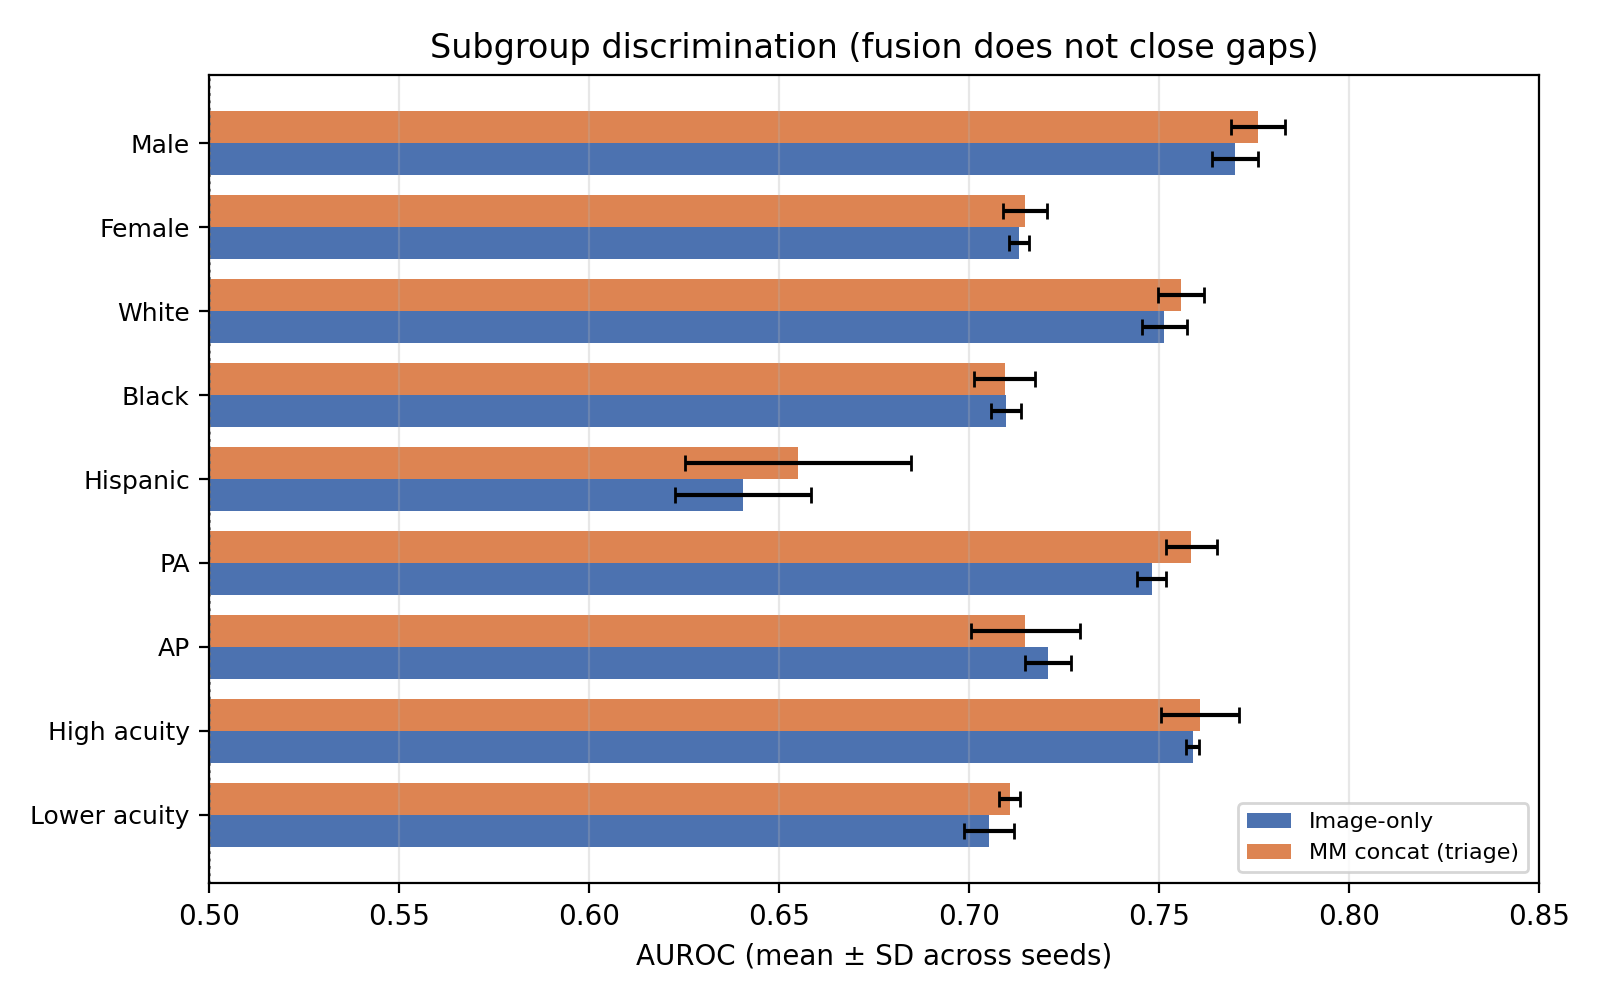
\includegraphics[width=0.75\textwidth]{fig3_subgroup_auroc.png}
\caption{Subgroup AUROC (mean $\pm$ SD across seeds) for image-only vs concat fusion; fusion
does not close sex, race or view gaps.}
\label{fig:subgroup}
\end{figure}

\begin{figure}[htbp]
\centering
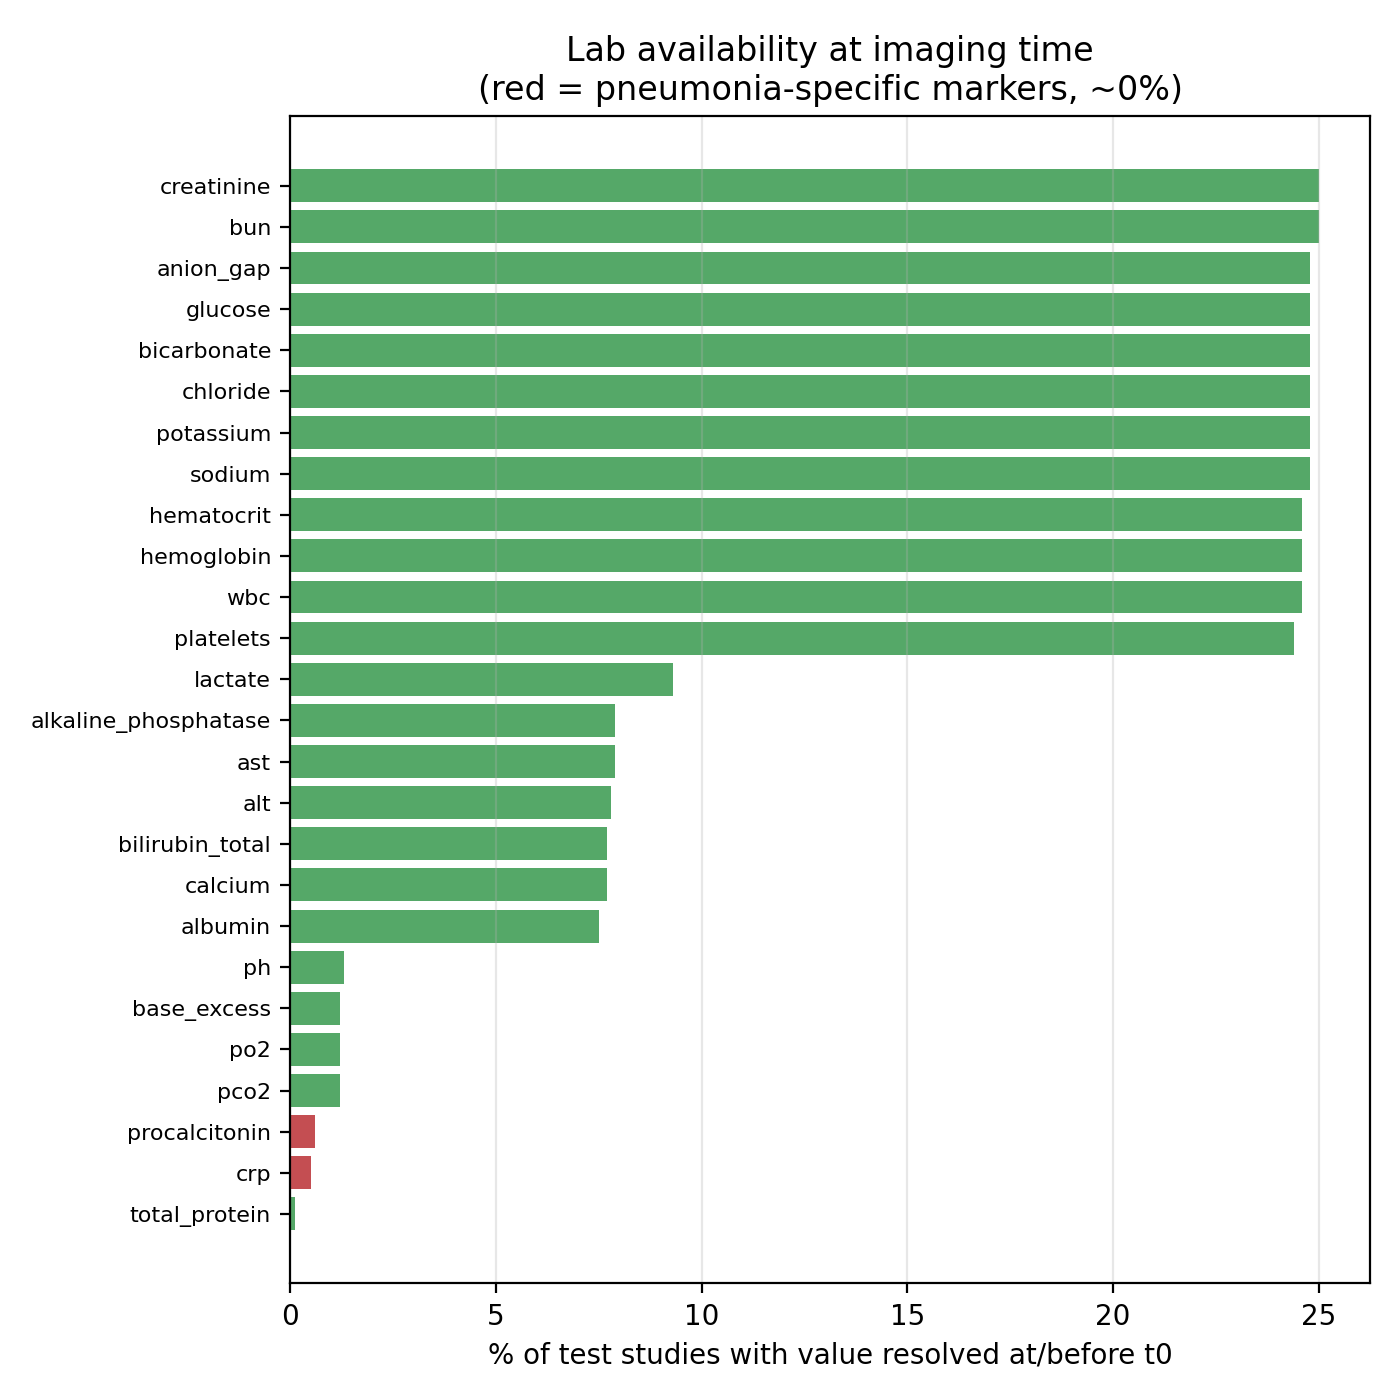
\includegraphics[width=0.62\textwidth]{fig4_lab_coverage.png}
\caption{Fraction of test studies with each lab resolved at or before $t_0$; pneumonia-specific
markers (red) are essentially unavailable at imaging time.}
\label{fig:labcov}
\end{figure}

\begin{figure}[htbp]
\centering
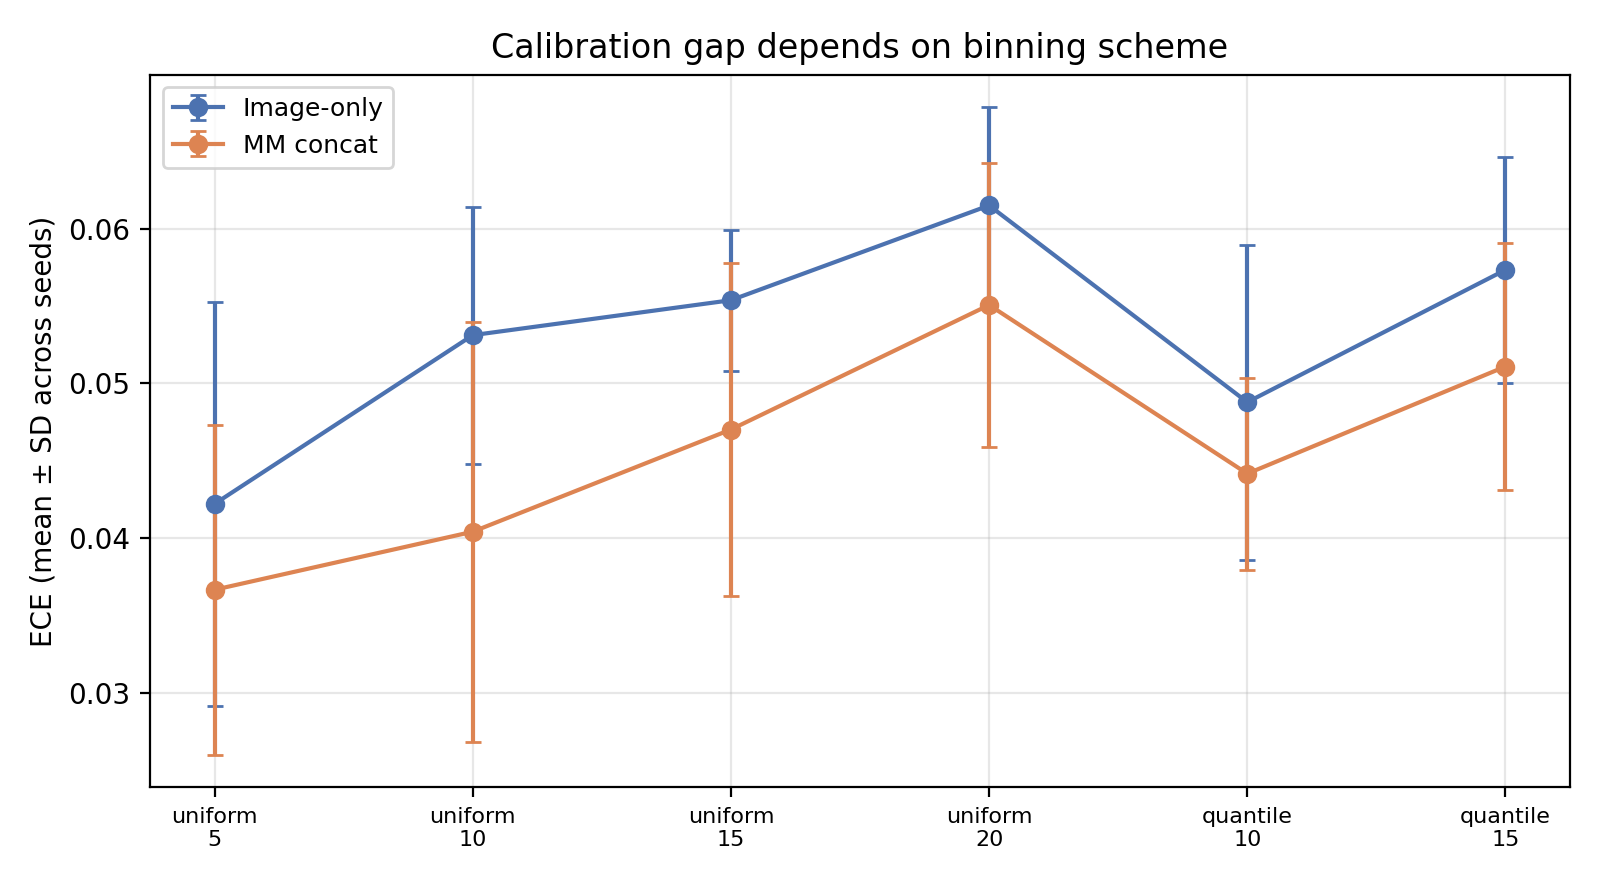
\includegraphics[width=0.8\textwidth]{fig5_ece_bin_sensitivity.png}
\caption{ECE under different binning schemes; the image--concat calibration gap depends on the
binning choice.}
\label{fig:ece}
\end{figure}

\section*{Data and code availability}
All results derive from scripts in the project repository, tied to the named temporal split:
cohort construction (\texttt{scripts/run\_data\_pipeline.sh}), multi-seed training and
aggregation (\texttt{scripts/multiseed/}) and analyses (\texttt{scripts/analysis/}). MIMIC and
NIH ChestX-ray14 data are publicly available (MIMIC via PhysioNet credentialing); no
patient-level data are redistributed.

\bibliographystyle{unsrtnat}
\bibliography{references}

\end{document}
